\documentclass[a4paper,oneside,12pt]{report}
\setlength\textwidth{155mm}
\setlength\textheight{247mm}
\setlength\topmargin{-10mm}
\setlength\headheight{0mm}
\setlength\oddsidemargin{05mm}
\setlength\evensidemargin{05mm}
\let\openright=\clearpage


%% Vytváříme PDF/A-2u
\usepackage[a-2u]{pdfx}

%% Přepneme na českou sazbu a fonty Latin Modern
\usepackage[czech]{babel}
\usepackage[utf8]{inputenc}
\usepackage{lmodern}
\usepackage[T1]{fontenc}
\usepackage{textcomp}


\usepackage{amsmath}						% rozšíření pro sazbu matematiky
\usepackage{amsfonts}						% matematické fonty
\usepackage{amsthm}							% sazba vět, definic apod.
\usepackage{bbding}							% balíček s nejrůznějšími symboly (čtverečky, hvězdičky, tužtičky, nůžtičky, ...)
\usepackage{bm}									% tučné symboly (příkaz \bm)
\usepackage{graphicx}						% vkládání obrázků
\usepackage{fancyhdr}						% možnost stylizovat záhlaví
\usepackage{fancyvrb}						% vylepšené prostředí pro strojové písmo
\usepackage{indentfirst}				% zavede odsazení 1. odstavce kapitoly
\usepackage[nottoc]{tocbibind} 	% zajistí přidání seznamu literatury,
\usepackage{icomma}         		% inteligentní čárka v matematickém módu
\usepackage{dcolumn}        		% lepší zarovnání sloupců v tabulkách
\usepackage{booktabs}       		% lepší vodorovné linky v tabulkách
\usepackage{paralist}       		% lepší enumerate a itemize
\usepackage{caption}						%	popisky
\usepackage{dirtree}						% strom souborů
\usepackage{minted} 						% vkládání kódu
\usepackage[bottom]{footmisc}  	% poznámky pod čarou vespod
\usepackage{bibentry} 					% citace přes celé heslo, používáno u první citace z jednoho zdroje
\usepackage{xurl}								% umožní url zalomit všude
\usepackage{hyperref} 					% odstranění červených okrajů v obsahu
\nobibliography*

\usepackage{color}
\usepackage{natbib}

\definecolor{pblue}{rgb}{0.13,0.13,1}
\definecolor{pgreen}{rgb}{0,0.5,0}
\definecolor{pred}{rgb}{0.9,0,0}
\definecolor{pgrey}{rgb}{0.46,0.45,0.48}
\renewcommand{\baselinestretch}{1.5}
%%% Údaje o práci

\def\NazevSkoly{Gymnázium, Praha 6, Arabská 14}
% Název oboru včetně počátečního 'Obor'.
\def\NazevOboru{Programování}

% Název práce v jazyce práce (přesně podle zadání)
\def\NazevPrace{Bezpilotní letadlo}

\def\NazevPraceShort{Bezpilotní letadlo}
% Název práce v angličtině
\def\NazevPraceEN{Drone}

% Název práce v němčině
\def\NazevPraceDE{Drohne}

% Jméno autora
\def\AutorPrace{Havránek Kryštof}

% Rok odevzdání
\def\RokOdevzdani{2022}
% Měsíc odevzdání
\def\MesicOdevzdani{Únor}

% Vedoucí práce: Jméno a příjmení s~tituly
\def\Vedouci{ing. Daniel Kahoun}

% Nepovinné poděkování (vedoucímu práce, konzultantovi, tomu, kdo
% zapůjčil software, literaturu apod.)
\def\Podekovani{%
\textbf{Poděkování}
}

% Abstrakt (doporučený rozsah cca 80-200 slov; nejedná se o zadání práce)
\def\Abstrakt{%
}

\def\AbstraktEN{%
}
\def\AbstraktDE{%
}
% 3 až 5 klíčových slov (doporučeno), každé uzavřeno ve složených závorkách
\def\KlicovaSlova{%
	(UAV), (Gtk), (C++), (Raspberry zero 2)
}
\def\KlicovaSlovaEN{%
	(UAV), (Gtk), (C++), (Raspberry zero 2)
}
\def\KlicovaSlovaDE{%
	(UAV), (Gtk), (C++), (Raspberry zero 2)
}

%% Balíček hyperref, kterým jdou vyrábět klikací odkazy v PDF,
%% ale hlavně ho používáme k uložení metadat do PDF (včetně obsahu).
\hypersetup{unicode}
\hypersetup{breaklinks=true}
\hypersetup{pdfborder=0 0 0}

%% Definice různých užitečných maker (viz popis uvnitř souboru)
\include{makra}

%% Titulní strana a různé povinné informační strany
\fancypagestyle{plain}{
\fancyhf{}
\renewcommand{\headrulewidth}{0.4pt}
\renewcommand{\footrulewidth}{0.4pt}
\fancyhead[C]{}
\fancyhead[L]{Ročníková práce -- \NazevSkoly}
\fancyhead[R]{\NazevPraceShort}
\fancyfoot[L]{Vypracoval: \AutorPrace	(\NazevOboru)}
\fancyfoot[C]{}
\fancyfoot[R]{\thepage}
}



\begin{document}

%%% Titulní strana práce

\pagestyle{empty}
\hypersetup{pageanchor=false}

\begin{center}

{\LARGE\bfseries\NazevSkoly}

\vspace{-18mm}
\vfill

{\LARGE\NazevOboru}

\vfill

\centerline{\mbox{\def\svgwidth{\columnwidth}\scalebox{0.25}{\input{../img/logo.pdf_tex}}}}

\vspace{-8mm}
\vfill

{\bf\Large ROČNÍKOVÝ PROJEKT}

\vfill


\vspace{15mm}

{\LARGE\bfseries\NazevPrace}


\vfill


Vypracoval: \hfill \AutorPrace

Vedoucí práce: \hfill \Vedouci

\vspace{15mm}
\MesicOdevzdani \ \RokOdevzdani

\end{center}



\newpage
\hypersetup{pageanchor=true}
\pagestyle{plain}
\pagenumbering{roman}


\openright


\vspace*{\fill}


\noindent
Prohlašuji, že jsem jediným autorem tohoto projektu, všechny citace jsou
řádně označené a všechna použitá literatura a další zdroje jsou v práci uvedené.
Tímto dle zákona 121/2000 Sb. (tzv. Autorský zákon) ve znění pozdějších předpisů uděluji
bezúplatně škole Gymnázium, Praha 6, Arabská 14 oprávnění k výkonu práva na rozmnožování díla
(§ 13) a práva na sdělování díla veřejnosti (§ 18) na dobu časově neomezenou a bez omezení
územního rozsahu.


\vspace{1cm}

\noindent
V ........ dne ............
\hspace{4cm}
Podpis autora


\newpage


\openright

\vbox to 0.20\vsize{
\setlength\parindent{0mm}
\setlength\parskip{5mm}

Název práce:
\NazevPrace

Autor:
\AutorPrace

% Vedoucí práce:
% \Vedouci, \KatedraVedouciho

Abstrakt:
\Abstrakt

Klíčová slova:
\KlicovaSlova

% Opakování v angličtině.
\noindent\rule{7cm}{0.4pt}

Title:
\NazevPraceEN

Author:
\AutorPrace

Abstract:
\AbstraktEN

Key words:
\KlicovaSlovaEN


% Opakování v němčině.
\noindent\rule{7cm}{0.4pt}

Titlel:
\NazevPraceDE

Autor:
\AutorPrace

Abstrakt:
\AbstraktDE

Schlüsselwörter:
\KlicovaSlovaDE

\vss}

\newpage

\openright



\tableofcontents


\newpage

\chapter*{Úvod}
\addcontentsline{toc}{chapter}{Úvod}

Cílem práce bylo sestavit bezpilotní letadlo a napsat doprovodný software -- a to jak pro samotný dron, tak počítač, který letadlo ovládá.
Uživatel sytému by měl mít možnost sledovat video stream z letadla a letadlo dálkově ovládat.
Programová část kódu by měla být psána v souladu s klasickými návrhovými vzory a umožňovat jednoduchou implementaci dalších funkcí.

Dron je postavený okolo malého počítače Raspberry Pi Zero 2, ke kterému jsou připojeny ostatní periférie přes sériovou a I2C linku.
Komunikace mezi dronem a pilotem probíhá přes TCP protokol.
Raspberry Pi tak funguje jako Access Point.
Konfigurační soubory pro nastavení Access Pointu jsou přiložené u kódu.

Celý kód práce je dostupný na Github pod licencí MIT -- \url{https://github.com/havrak/UAV-project}.
V rámci práce na projektu byly napsány tři doprovodné knihovny -- \url{https://github.com/havrak/Raspberry-JY901-Serial-I2C}, \url{https://github.com/havrak/raspberry-pi-ina226} a \url{https://github.com/havrak/PCA9685-rpi}.
Všechny jsou volně dostupné k použití také pod licencí MIT.



\pagenumbering{arabic}
\setcounter{page}{1}

\chapter{Rozložení práce}

Práci lze rozdělit na dva základní komponenty.
První část software běží na počítači přes který se bezpilotní letadlo ovládá, druhá na samotném dronu.
Obě části jsou psané v jazyce C++.

Software pro počítač používá grafickou knihovnu Gtk3 a byl vyvíjen primárně na operačním systém Linux.
Gtk3 je multiplatformní toolkit, port na další operační systémy je tak možný a kód je psán stylem, aby umožnil další verze.

Jádro samotného dronu představuje malý počítač Raspberry Pi Zero 2.
Vyšší výkon verze Zero 2 není nutný pro fungování, práce tak defacto může fungovat na libovolném Raspberry Pi.
Program využívá jen zlomek zdrojů arduino a to jak po stránce paměti, tak výpočetního výkonu.

Obě části mezi sebou komunikují prostřednictvím protitoku založené na TCP rodině.
Přenos videa je zprostředkovávám pomocí UDP.
Samotné video je kódováno do jpg, v porovnání s dalšími styly přenosu byla latence u jpg menší.

\section{Komunikační protokol}

Ovládací počítač a Raspberry mezi sebou komunikují prostřednictvím jednoduchého TCP protokolu.
Raspberry Pi přebírá na sebe roli serveru, to mimo jiné umožňuje aby bylo zařízení ovládáno z více stanic.
Případně alespoň telemetrie byla posílána na více zařízení.

Protokol prozatím není zašifrovaný a nepočítá s nevalidními daty.
Šifrován není příliš nutné, dronu a počítač operují na vlastní síti, kde Raspberry Pi funguje jako Wi-Fi Access--Point.
Struktura protokolu ovšem nabízí možnost jednoduše naimplementovat symetrickou kryptografii.

\subsection{Struktura protokolu}

Každý packet začíná hlavičkou o velikosti 5 bytů.

\begin{enumerate}
	\item typ zprávy
	\item priorita -- Program prozatím prioritu nebere v potaz.
	\item 8 horních bitů velikosti zprávy
	\item 8 dolních bitů velikosti zprávy
	\item dopočet do kontrolního součtu -- součet čísel v hlavničce musí být dělitelný sedmi.
\end{enumerate}

Po hlavičce následuje samotná zpráva zakončená posloupností pěti bytů -- 0x00, 0x00, 0xFF, 0xFF, 0xFF.
Zakončovací řetězec slouží pro případ, kdy nějaký packet nedorazí, či příchozí zpráva byla nějak poškozena.
Nastane li tato situace program postupně čte byty ze socketu a hledá tuto sekvenci.
Maximální délka zprávy je půl kilobytu, samotná data jsou posílána v balíčcích o maximální velikosti 250 bytů.
Omezení velikosti zprávy je zavedeno hlavně kvůli šetření paměti -- program má pro každého klienta vytvořené jedno pole, do kterého se musí vejít celá zpráva.

Protokol funguje na základě posílání struktur, definovaných v  \verb|protocol_spec.h|.
Pro odeslání dat je nejprve nutné nahrát data do struktury.
Dále se z těchto dat vytvoří tzv. SendingStructure, které se odešle do thread pool.
Pro přijetí se data načítají do bufferu spojeným s klientem, ze kterého se později zkopírují objektu ProcessingStructure.
Příslušná část programu si pak data přes memcpy opět zkopíruje na příslušnou strukturu.

Pro příjem a zpracování zpráv slouží dva thread pooly -- SendingThreadPool a ProcessingThreadPool.
Jednotlivé části programu tak nemusí čekat až se uvolní socket aby se mohla data odeslat, či čekat na jejich zpracování pro přijetí.
Speciální případem je zpracování příkazů, které přímo ovládají pohyb letadla.
Pro ovládaní existuje samostatné vlákno, které příkazy vykonává sekvenčně.
Také je implementován mechanismus, kde příliš staré příkazy se nevykonají.

Program sleduje aktivitu na socket pomocí příkazu select.
Při běžné provozu tak většina vláken komunikací spí a zátěž není příliš velká.

z hlediska programové stránky jsou veškeré součásti komunikace implemetovány jako singletony.
Program je tak řešen, aby umožnil jednoduše odesílat zprávy z různých částí programu.

\subsection{Specifikace protokolu}

Protokol obsluhuje tři základní části provozu dronu -- nastavení, ovládaní a telemetrie.
Pro nastavení je vyhrazen rozsah od 0x00 po 0x20 a zahrnuje věci jako odpojení klienta, nastavení kamery, či restart.

Další kategorii představuje ovládaní, pro které je vyhrazen prostor mezi 0x21 až 0x40.
Projekt implementuje dva základní typy -- standardní ovládaní (pohyb joysticku, atd.) a speciální.
Standardní slouží pro prosté manuální ovládání dronu.
Speciální například resetuje polohoměr, či zapíná autopilota.

Poslední kategorií je telemetrie, které má zbytek rozsah do 0xFF.
Tu ve standardním chování posílá Raspberry každých pár stovek milisekund.
Chce li client aktuálnější data může si je vyžádat odesláním zprávy o stejném typu, jako jsou požadovaná data.
Speciální případ představují chybové hlášky, které vyžádat pochopitelně nejdou a pilotovi se zobrazují v dialogovém okně.

\chapter{Hardware a Raspberry Pi}

Jádro samotného letadla tvoří malý počítač Raspberry Pi Zero 2.
Ostatní periférie jsou: polohový senzor WT901B, voltmetr a ampérmetr INA226, ovladač na serva PCA9865, ublox NEO-7M GPS modul a BEATLES 40A ESC.
Vše s výjimkou GPS komunikuje s Raspberry Pi prostřednictví I2C protokolu.
GPS modul pak pomocí sériové linky.

Senzor WT901B sice podporuje přímé napojení GPS senzoru, při pokusu o konfiguraci senzoru však přestala fungovat sériová komunikace obecně.
GPS je tak napojena sólo.

Systém má dva přívody proudu -- hlavní motor a serva jsou napájeny prostřednictví ESC.
To však nebylo schopné poskytovat dostatečný proud pro Raspberry Pi a senzory na něj napojené.
Z baterie je tak vyvedená linka napojená na step down converter, který 14.8 V sníží na 5V.
Ty jsou přímo napojeny na Raspberry Pi.

\begin{figure}[h]
	\centering
	\includegraphics[height=12cm]{../img/schema.png}
	\caption[Schéma zapojení obvodu]{Schéma zapojení obvodu}
\end{figure}

\newpage

\begin{figure}[h]
	\centering
	\includegraphics[height=9cm]{../img/circuit.jpg}
	\caption[Reálné zapojení]{Reálné zapojení\footnotemark}
\end{figure}
\footnotetext{TP-LINK WN772N je aktuálně volně vedle Raspberry Pi, nikoliv pod}

Většina komponentů je napájena na bread board, který lze jednoduše nasadit na Raspberry Pi.
Výjimku představuje voltmetr/ampérmetr, který je volně a v letadle se nachází v ocase.
Ke zbytku se připojuje přes koncovku USB, ostatní koncovky jsou XT60.
V aktuální verzi je zapojení relativně nepraktické -- z ocasu do přídě vedou tři kabely.

\begin{figure}[h]
	\centering
	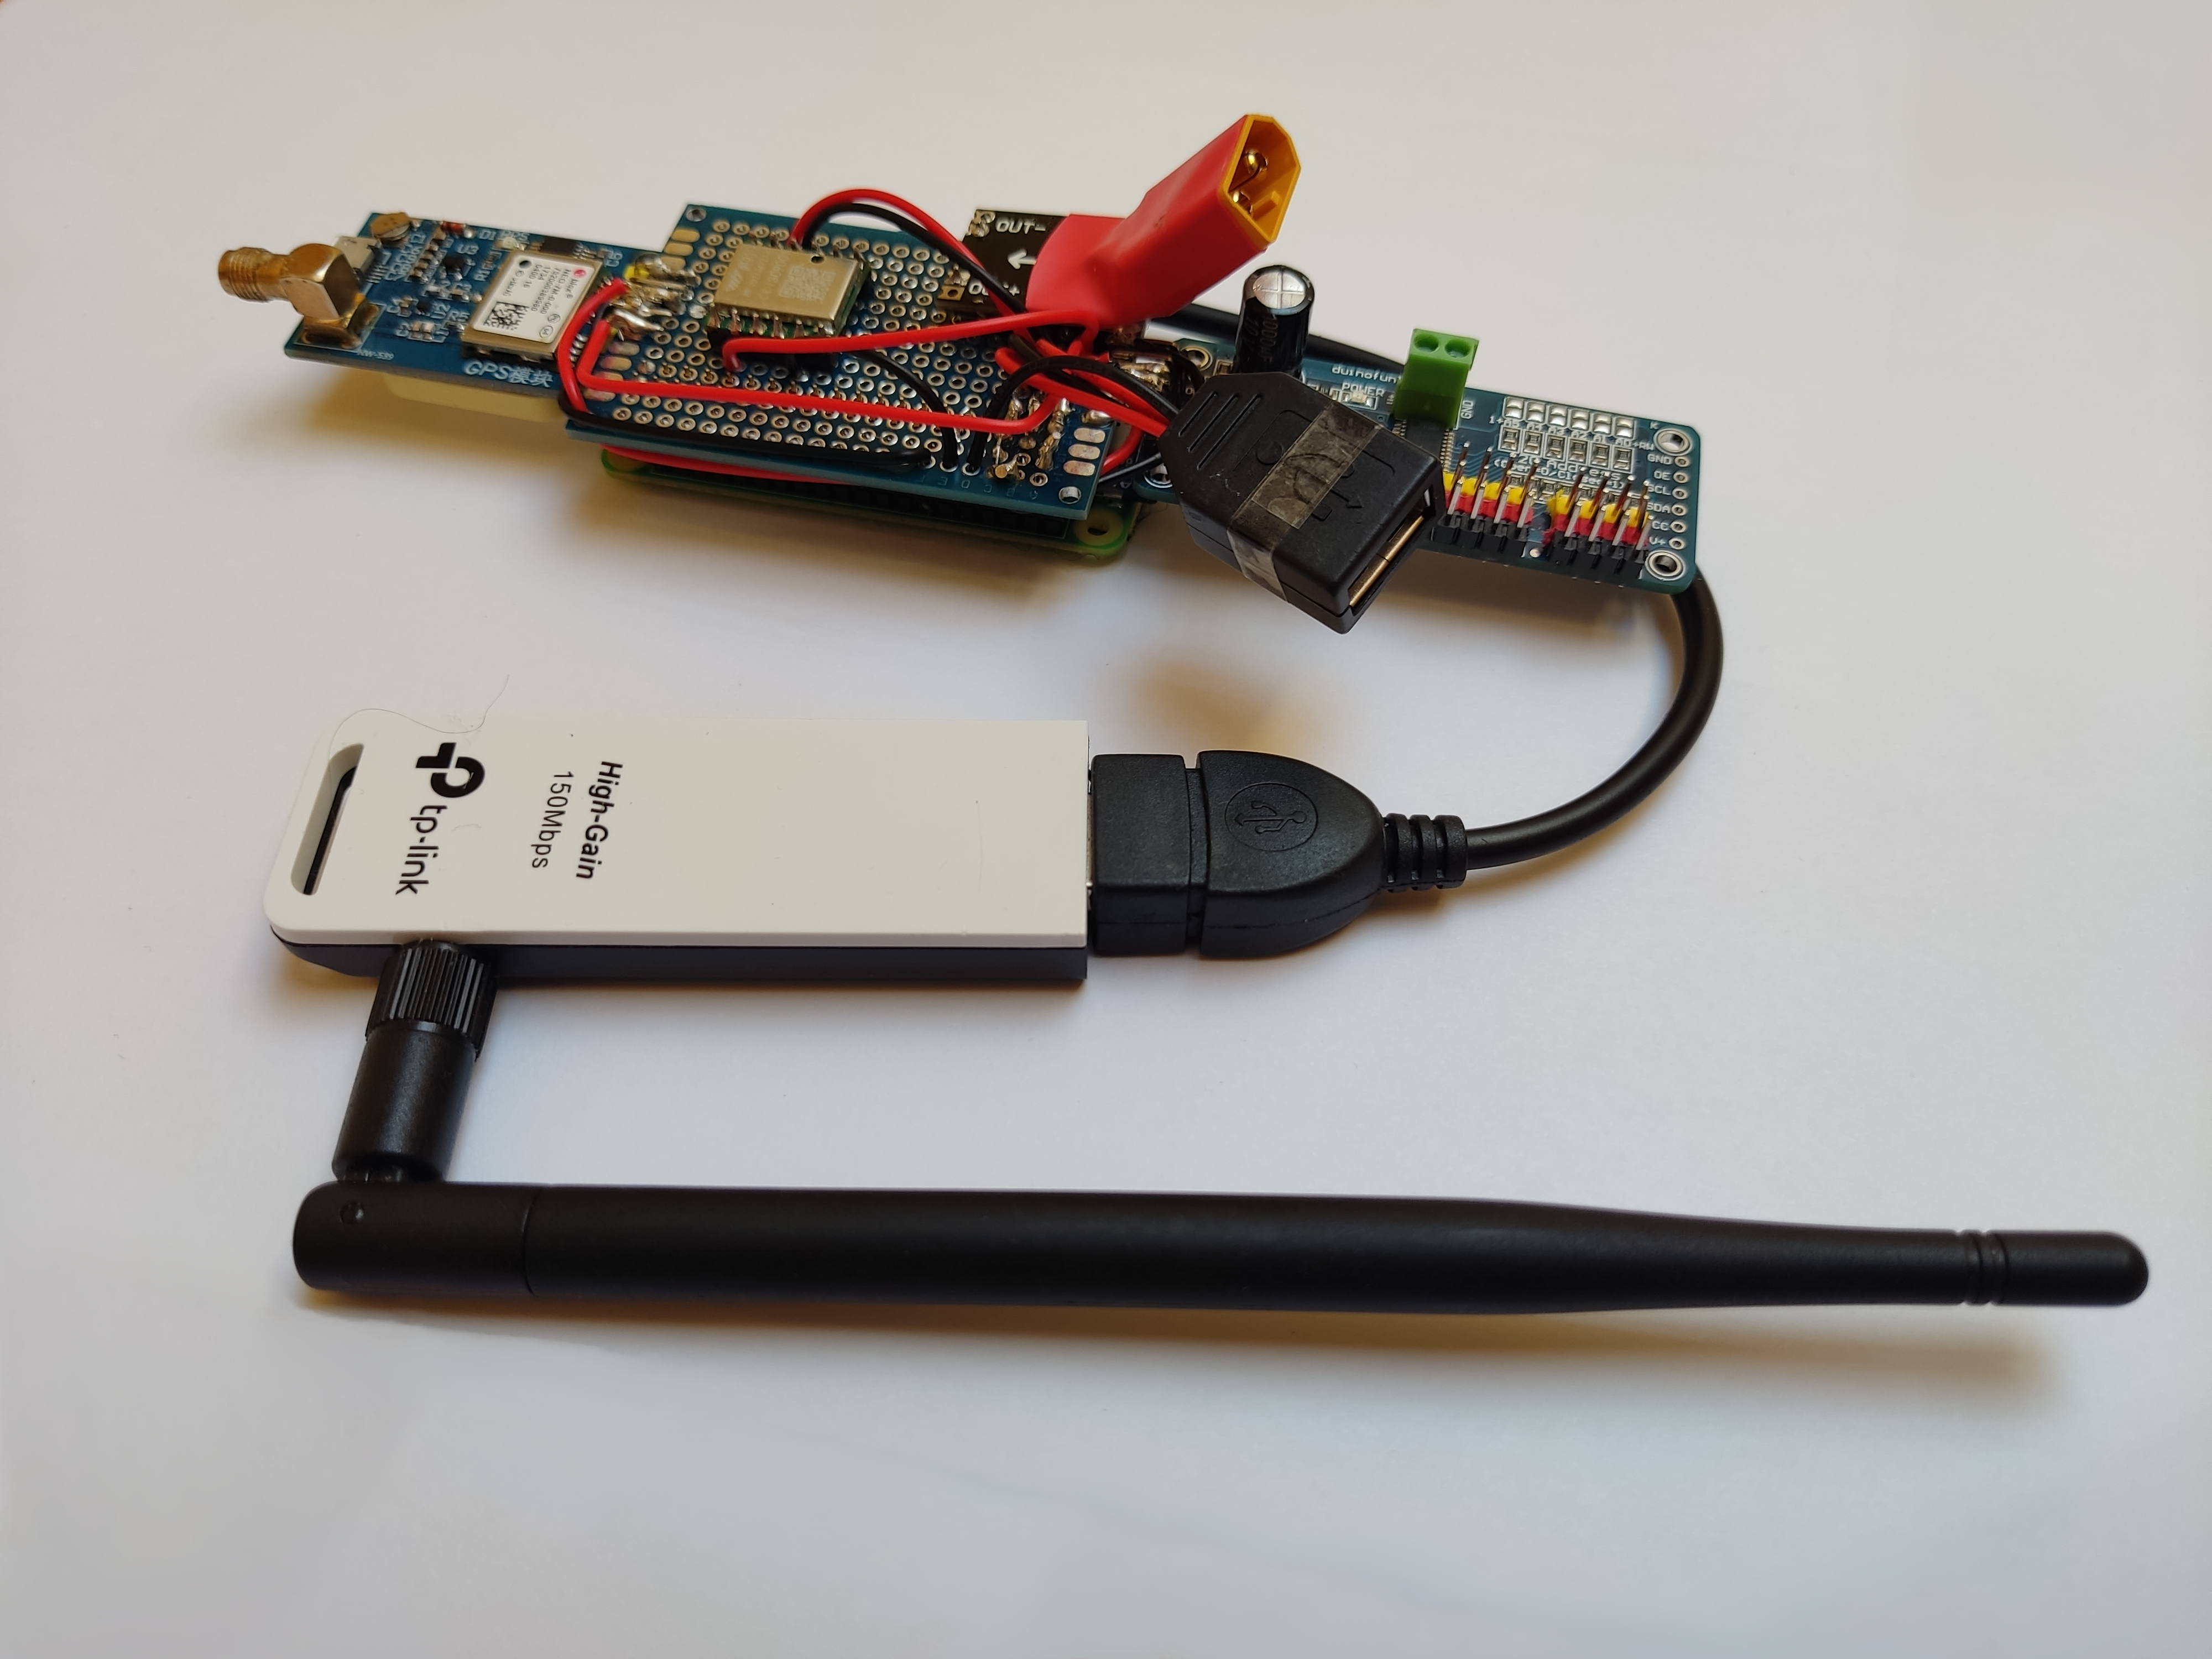
\includegraphics[height=7cm]{../img/detail.jpg}
	\caption[Detail Raspberry Pi]{Detail Raspberry Pi}
\end{figure}


\newpage

\begin{figure}[h]
	\centering
	\includegraphics[height=6cm]{../img/body.jpg}
	\caption[Detail těla dronu]{Detail těla dronu}
\end{figure}

\begin{figure}[h]
	\centering
	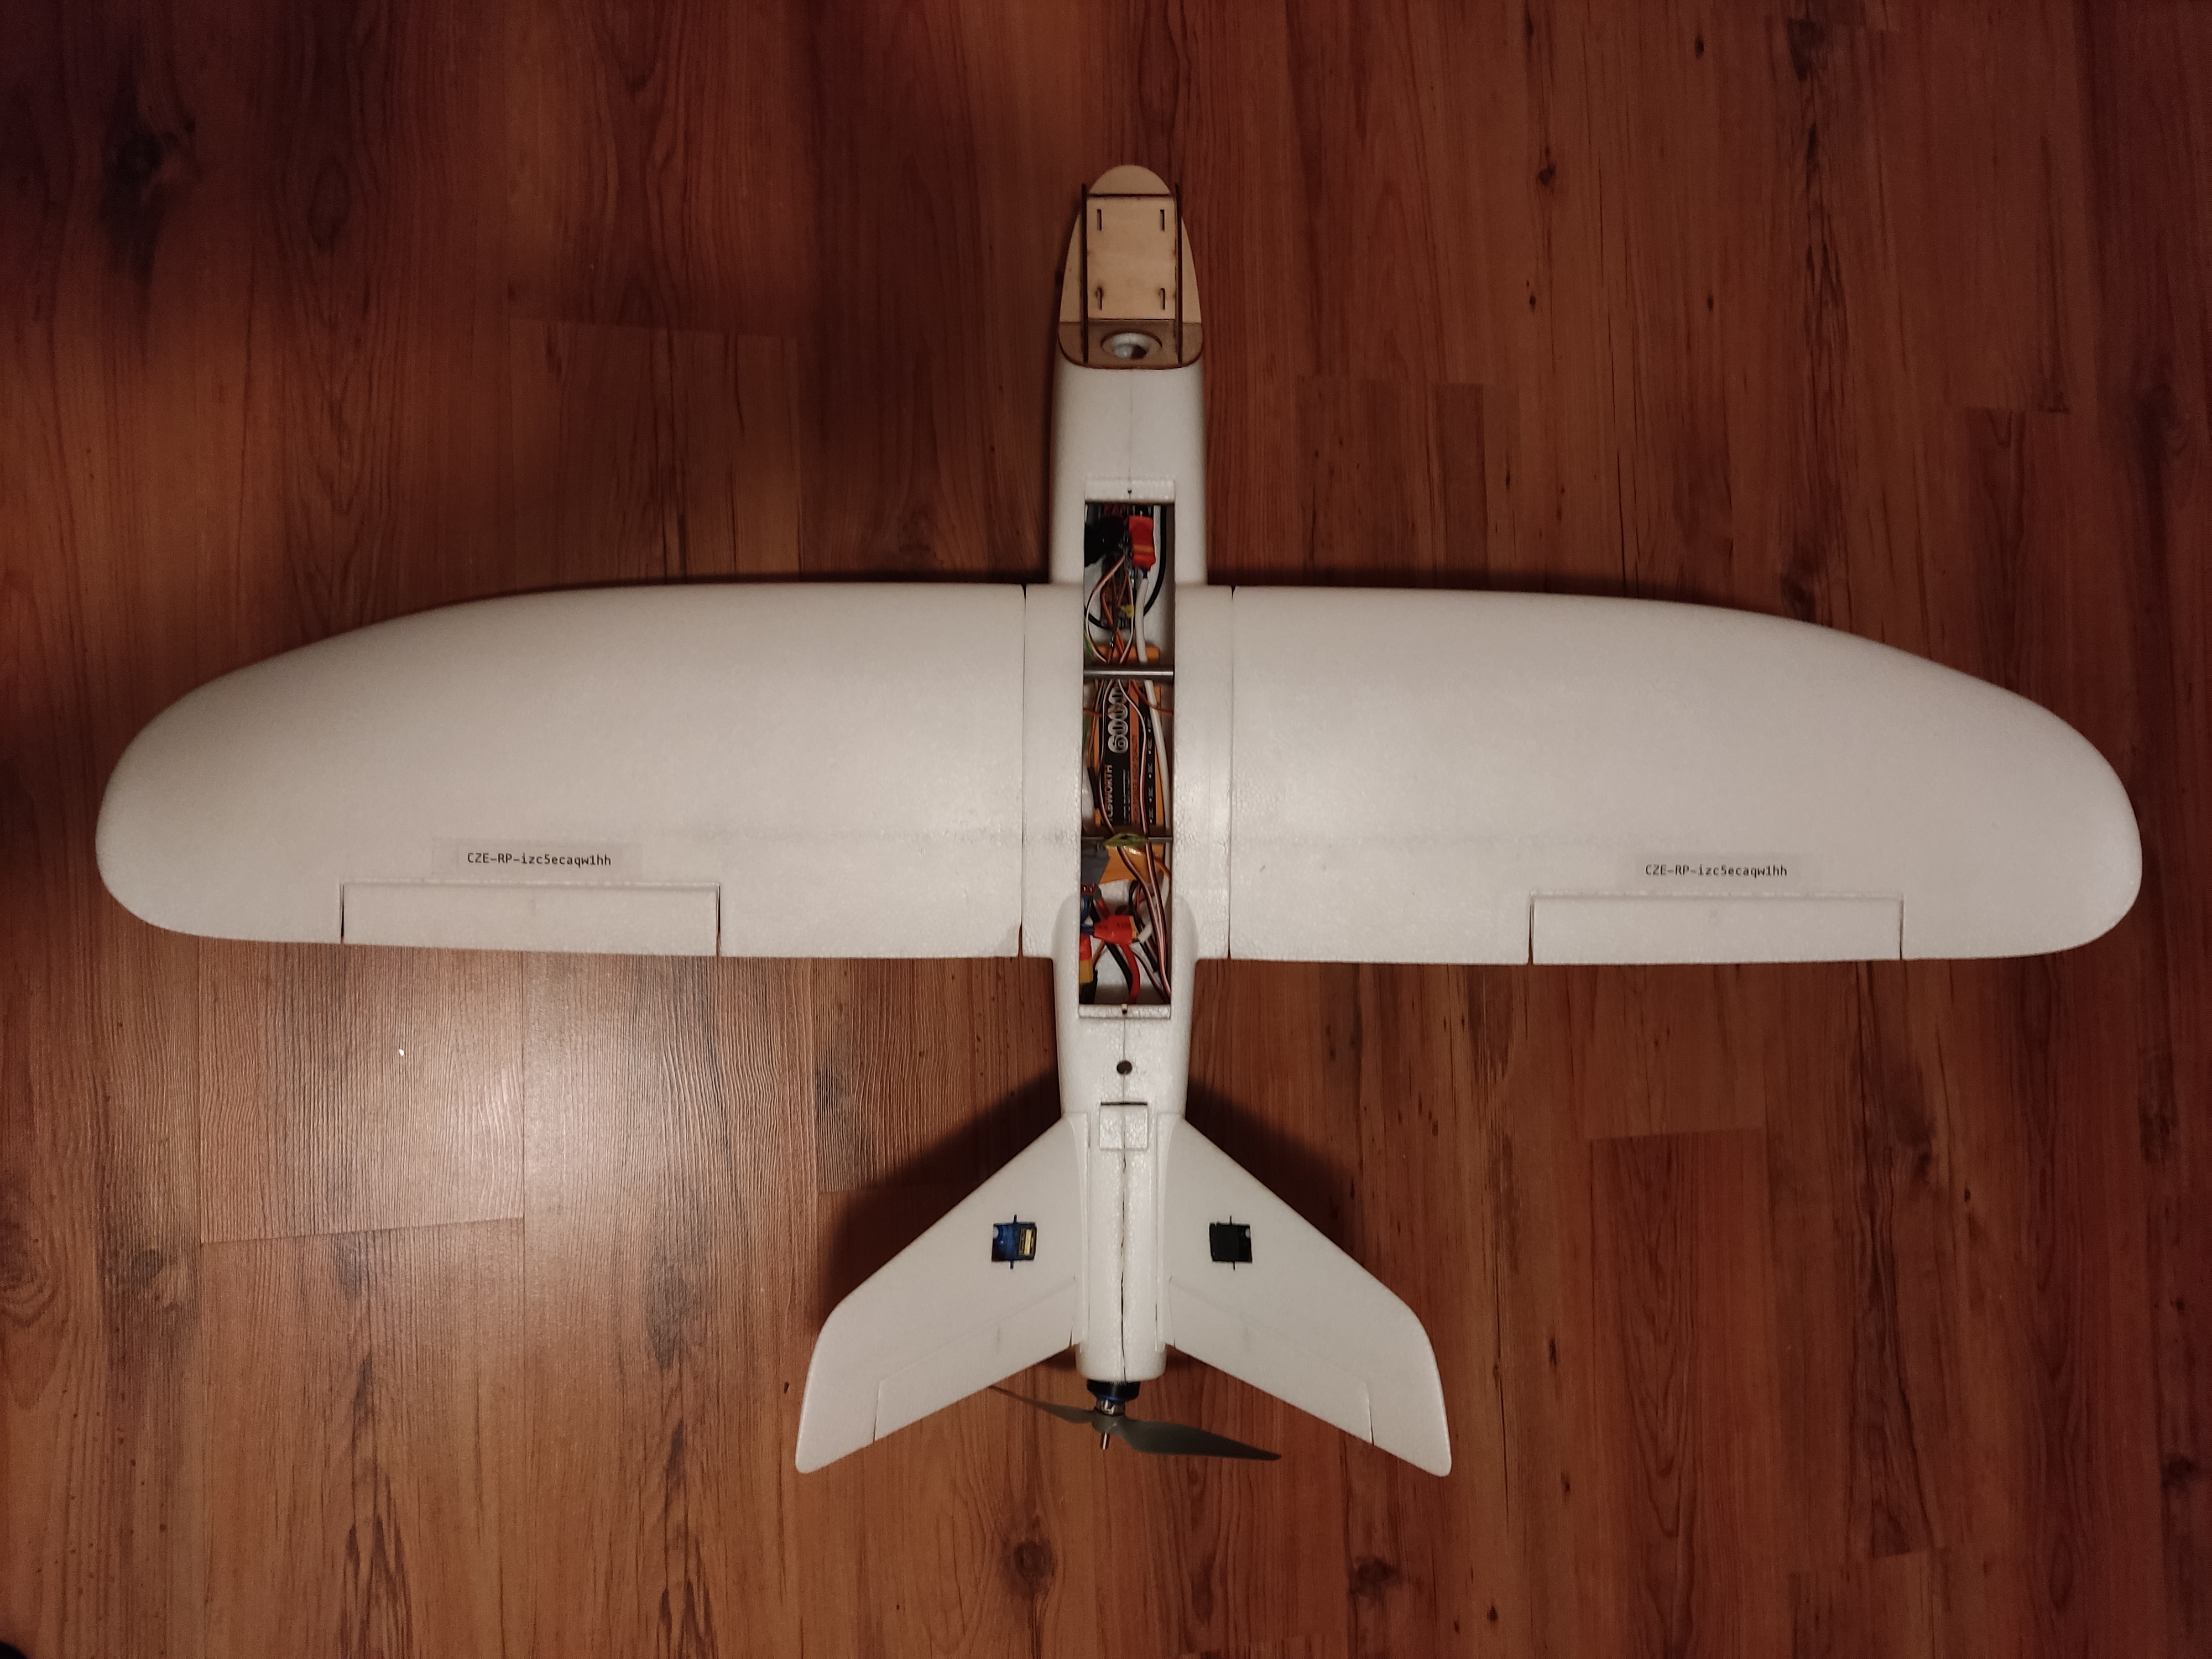
\includegraphics[height=10cm]{../img/whole_plane.jpg}
	\caption[Celý dron]{Celý dron}
\end{figure}


Kostrou dronu je model Mini Talon od čínské společnosti X-UAV.
Rozpětí křídel je 130cm délka pak 85cm.
Jedná se o tzv. V-Tail konfiguraci ocas tedy nemá standardní tři kontrolní plochy ale pouze dvě.
V aktuální verzi program má naimplementované ovládání pouze pro tuto konfiguraci.

\newpage

\section{Program}

\begin{figure}[h]
	\dirtree{%
		.1 drone\_software.
		.2 libraries.
		.3 Raspberry-JY901-Serial.
		.3 raspberry-pi-ina226.
		.3 rpidmx512-Lib-PCA9685.
		.2 include.
		.3 battery\_interface.h.
		.3 camera\_streamer.h.
		.3 communication\_interface.h.
		.3 generic\_PID.h.
		.3 gps\_interface.h.
		.3 imu\_interface.h.
		.3 protocol\_spec.h.
		.3 servo\_control.h.
		.3 telemetry.h.
		.2 src - implemetation of  header files.
	}
	\caption[Struktura souborů frontendu, vlastní tvorba]{Struktura souborů frontend}
	\label{fig:frontendStructure}
\end{figure}

Program na Raspberry Pi používá tři základní knihovny pro komunikaci s WT901B, INA226 a PCA9685.
Přenos z kamery pak zprostředkovává OpenCV, který jako backend používá gstreamer.
V budoucnu je tak možné přidat zpracování videa přímo na raspberryPi -- například detekce věcí na obrazu.

\section{Interface s Hardwarem}

Jak už bylo řečeno s hardwarem Raspberry komunikuje prostřednictví I2C spojení a sériové linky.
Pro zpracování dat z INA226 a WT901B byly napsány nové knihovny.
Jelikož knihovny pro Raspberry Pi totiž buďto neexistovaly, nebo nebyly zdaleka kompletní.

Knihovna pro WT901B vznikla forkem knihovny pro Arduino\footnote{\bibentry{WT901BL}} a byla předělána v souladu s dokumentací protokolu\footnote{\bibentry{WT901B}}
Kvůli problémům se seznorem byla i dopsána I2C komunikace, kterou původní knihovna neimplementovala

 případě knihovny pro INA226 bylo forknuto demo\footnote{\bibentry{INA226L}} a dopsáno v plnohodnotnou knihovnu.

Obě knihovny využívají knihovnu wiringPi.
Ta byla koncem roku 2021 spolu s vydáním raspbian bullseye označena ze deprecated.
Také dochází ke kolizím mezi částmi kódu, které přistupují k I2C přes knihovnu WiringPi a částmi kódu, které přistupují přímo přes bcm2835.
Nejedná se o kritickou chybu, ale někdy je narušena integrita některých dat.

Vzhledem k přímočarosti výstupu z GPS modulu je celá implementace přímo součástí hlavního kódu.
Program zpracovává GPGGA packet, který obsahuje veškerá důležitá data.
Zpracování dalších packetů nebylo pro práci podstatné.

V neposlední řadě k PCA9685 se také přistupuje přes knihovnu\footnote{\bibentry{PCA9865}}.
Knihovna je v základu psána pro Raspberry Pi a implementuje všechny funkce potřebné v projektu.

\section{Organizace v kódu}

Z programu se k perifériím přistupuje přes několik singletonů -- ImuInterface pro WT901B, BatterInterface pro INA226, GPSInterface pro ublox NEO 7M a ServoControl pro PCA9865.
Důvod řešení přes singletony je opět stejný jako u komunikace.
Data ze senzorů jsou potřeba v různých částech programu a reálně reprezentují pouze jeden senzor.

Funkce tak nemusí mít celou řadu parametrů a program nepotřebuje jednu centrální třídu, která bude vše organizovat.
Mizí tak i problémy s řadou lokálních proměnných a nutností je udržovat aktuální.
Jelikož celý program je více vláknový implementují tak singletony ochranu před kolizí několika vláken a vzniku nevalidních dat.

Data ze senzorů, jsou také agregována v třídě telemetry.
Ta se stará o nastavení všech senzorů a pak zajišťuje vytvoření packetů pro odeslání klientovi.
Ze stejných důvodů jako další třídy i telemetry je implementována jakožto singleton.

O přístup ke kameře se stará třída CameraStreamer.
Ta se vytváří dynamicky na základě požadavku od klienta.
Jelikož aktuálně není implementována žádná analýza obrazu z kamery přímo na Raspberry Pi proces stremu vznikne jako fork procesu ve kterém je spuštěn stream.
Jelikož se jendá o fork při ukončení rodičovského procesu se ukončí i stream a program samotný se o přenos nemusí nijak starat.

\section{Ovládání letadla}

O ovládání kontrolních ploch a motoru se stará třída ServoControl.
V aktuální podobě přímo zpracovává data z ovladače, která posílá server.
Není tak možné jednoduše změnit jaké ovládací prvky budou jak ovládat letadlo.A

Na počátku zpracování nových příkazů jsou hodnoty analogové páčky přepočítány do čtvercové plochy.
Standardně se totiž mapují ovladače na kruh -- páčka čistě nahoru tak má výrazně vyšší hodnotu osy Y, než páčka pod úhlem 45 stupňů, to i přesto, že urazily stejnou vzdálenost.
Bez této korekce tak ovládání působilo velmi neresponzivně, kdy praktické byly pouze polohy jih, sever, západ, východ.

V případě konfigurace ocasu do tvaru písmena V je interpretace ovládání relativně jednoduchá.
Ocasní plochy (Ruddervator) ovládání bočení a klopení.
Plochy na křídlech pak pouze klonění, teoreticky mohou ovládat i klopení, v tomto případě to však nebylo třeba.

\subsection{Autopilot}

Projekt implementuje i jednoduchého autopilota, který je schopen držet letovou hladinu.
Vyrovnávání řeší dva proporčně-integračně-derivační ovladače, které se snaží minimalizovat chybu.
Jeden minimalizuje odchylku v klopení, druhý pak odchylku v klonění.
Bočení minimalizovat není třeba -- pro bočení musí být letadlo nakloněno.

Teoreticky by mohlo jít tento sytém rozšířit aby se snažil minimalizovat odchylku nikoliv od původního směru, ale od pomyslného bodu určeného souřadnicemi GPS.
Letadlo by tak nejenže letělo více rovně (aktuálně je autopilot náchylní na změnu posunutí v příčné ose), ale mohlo samo doletět na specifikovaný bod.


\chapter{Client na ovládání}




\chapter*{}
\pagenumbering{roman}
\setcounter{page}{6} % text bude pokračovat v číslování římském, kde přestal na začátku souboru
\chapter*{Závěr}
\addcontentsline{toc}{chapter}{Závěr}

Cíl práce specifikovaný v zadání byl splněn.
Letadlo je schopné letu a uživatel má k dispozici stream z kamery na dronu.

Práci však komplikovala řada problémů a to jak s hardwarem, tak se softwarem.
Před začátkem jsem měl jen velmi povrchní zkušenosti s jazykem C++ a žádné s jak Gtk3, tak vývojem pro Raspberry Pi.
Práce tak nemohla být realizována tak, jak byla původně zamýšlena.

Tomu napovídá i dlouhý list specifikující budoucnost projektu.
Ačkoliv tomu samotné řádky kódu nemusí napovídat práce mi dala celou řadu nových znalostí.
I proto plánuji dále na projektu pokračovat ve svém volém čase.
Rád bych systém dostal do stavu kdy se jedná o plnohodnotnou realizaci bezpilotního systému.



\bibliographystyle{czplainnat}   %% Autor (rok) s českými spojkami
%\bibliographystyle{plainnat}    %% Autor (rok) s anglickými spojkami
%\bibliographystyle{unsrt}       %% [číslo]


\renewcommand{\bibname}{Seznam použité literatury}

\bibliography{literatura}

%%% Kdybyste chtěli bibliografii vytvářet ručně (bez bibTeXu), lze to udělat
%%% následovně. V takovém případě se řiďte normou ISO 690 a zvyklostmi v oboru.

% \begin{thebibliography}{99}
%
% \bibitem{lamport94}
%   {\sc Lamport,} Leslie.
%   \emph{\LaTeX: A Document Preparation System}.
%   2. vydání.
%   Massachusetts: Addison Wesley, 1994.
%   ISBN 0-201-52983-1.
%
% \end{thebibliography}



\listoffigures
\openright
\end{document}
